\documentclass[11pt, a4paper,oneside]{report}
\usepackage[left=3cm,right=3cm,top=3cm,bottom=3cm]{geometry}
\usepackage{setspace}
\onehalfspacing

\newcommand{\mychapter}[2]{
    \setcounter{chapter}{#1}
    \setcounter{section}{0}
    \chapter*{#2}
    \addcontentsline{toc}{chapter}{#2}
}
\usepackage{verbatim}
\usepackage{graphicx}
\usepackage{multirow}
\usepackage{subfigure}
\begin{document}

\title{Evolutionary innovation in eukaryotic proteins}
\author{Oxana Sachenkova}
\date{}
\maketitle

\mychapter{0}{Introduction}
More than 150 years after the publication of Darwin's {\itshape Origin of Species}, we still struggle to understand the processes of evolution and how they shape the diversity of life on Earth. The application of the idea of "descent with modification" to the genome continues to produce fundamental insights into how biological systems evolve. Changes on the DNA level that occur due to recombination events, errors during meiosis and random mutations can change the proteins synthesized in our cells: their structures, expression levels, interactions and their emergent functions.  Analysis of protein evolution is essential for investigating important biological questions such as the evolution of speciation, identification of functionally important sites, drug targets or novel protein functions.
  
Advances in experimental methods such as fast and precise whole-genome sequencing, NMR-spectroscopy and mass spectrometry generate vast amounts of data about protein expression levels, protein structure and function in different organisms.  This large increase of genome-wide information provides new opportunities to study molecular evolution using computational and statistical approaches.

In this research project we are particularly interested in mechanisms of generating evolutionary novelty in protein structure and function. The interplay between gene duplication, insertion and deletion events, mutations and evolutionary constraints is our main focus.  Using computational methods such as protein structure prediction, multiple sequence alignment, machine learning and statistical data analysis we hope to shed light on some aspects of the mechanisms of evolution of novel protein function. Two main research questions I am focusing on are: How do long indels and duplications influence protein function? How do naturally unstructured proteins evolve in comparison with ordered proteins? 

\mychapter{1}{Background}

This chapter introduces the key concepts that are important for understanding the proposed research topic. 
\section{Basic terminology}
\subsection{Building blocks of life}
Cell is the smallest unit of living matter: it consumes energy to maintain its organization and is capable of reproducing itself. These properties are central to the definition of life. All known living organisms consist of one or multiple cells, and in all cases, the whole organism is generated by cell divisions from a single cell. The single cell, therefore, contains all the necessary information and machinery that defines the organism.  Since the discovery of Watson and Crick in 1953\cite{Watson1974} we know that all the living cells store this information in the form of double-stranded molecules of DNA - long unbranched paired polymer chains, formed always of the same four types of monomers, nucleic acids. These monomers, referred to as A, T, C and G are attached  in a linear sequence that encodes the hereditary information of the cell. Information stored in DNA is read out and put to use through a two step process: first, in transcription, segments of DNA sequence are used to guide the synthesis of many molecules of RNA, then, in translation some of the RNA molecules are used to synthesize the molecules of protein and some are helping with this process\cite{rRNA}.

 A certain set of rules for translating DNA to protein is shared between all of the living cell.  Different combinations of three base pairs in the DNA, named codons, code for a certain amino acid or serve as a signal of a start or end of a sequence.  This genetic code rule set is redundant, some codons can code for the same amino acid\cite{Turanov2009}. Each segment of DNA that encodes for a functional molecule, either RNA or protein is called a gene\cite{Gerstein2007}.  Complete set of DNA molecules of an organism, including all of its genes is called a genome.  

Protein molecules are long unbranched polymer chains, but they are formed by different monomeric building units, amino acids. Each protein molecule, or polypeptide, is created by joining amino acids in a particular sequence and then folding into a three-dimensional form with reactive sites on its surface. Proteins constitute more than 50\%  of the cell's dry mass\cite{Alberts2007} and perform nearly all the cell’s functions: catalyzing metabolic reactions, replicating DNA, responding to stimuli, and transporting molecules from one location to another.
\begin{figure}[hb]
\begin{center}
\label{img:dnatoprotein}
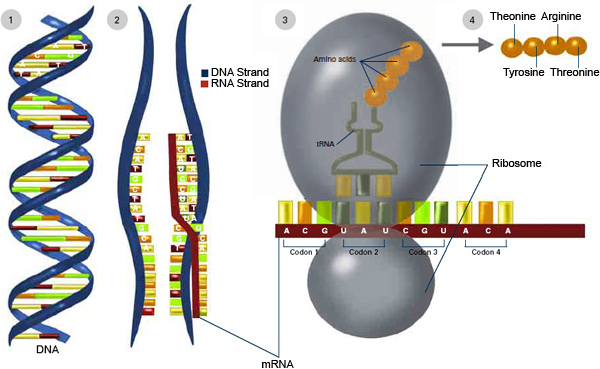
\includegraphics[width=0.8\textwidth]{figures/dna_to_protein.jpg}
\end{center}
\caption{1. RNA polymerase transcribes DNA to make messenger RNA (mRNA). 2. The mRNA sequence (dark red strand) is complementary to the DNA sequence (blue strand). 3. On ribosomes, transfer RNA (tRNA) helps convert mRNA into protein. 4. Amino acids link up to make a protein.} 
\end{figure}

\subsection{Three domains of life}
Considering their evolutionary descent and unique biochemistry of the cell living organisms are classified in three main branches: Archaea, Eukarya and Bacteria. The organisms of both Archaea and Bacteria consist of a single cell with a DNA not separated from the cytoplasm. DNA of Eukarya, in contrast, is packed in its own membrane-bound organelle called the nucleus. Some eukaryotes, like amoebae and yeast, are single-celled organisms. Other eukaryotic cells are part of multicellular organisms, including plants and animals. The three domains of life also demonstrate fundamental differences in genome organization and mechanisms of evolution. The genome of Bacteria is limited to 180kb - 13 Mb and Archaea to 500kb - 5 mb\cite{Koonin2008}, while that of eukaryotes can be characterized by a significant expansion in size\cite{Gregory2007} and complexity\cite{Parfrey2008}. Evolution of bacterial and archaea genomes involves two major processes: acquisition of exogenous DNA through horizontal gene transfer and genome decay through deletion\cite{Pal2005}. Eukaryotic cells demonstrate an increase in the amount of genetic information through such mechanisms as non coding DNA, gene duplication, alternative splicing, etc.  The genomes of Archaea are similar to Bacteria in size and gene density, but some tRNA gene sequences are interrupted by non translational sequences, called introns. This mechanism is also seen in eukaryotes. 
In this research project we will be focusing on studying the mechanisms of evolution in eukaryotic genomes. This domain of life is further subdivided into five kingdoms: Protozoa (unicellular eukaryotic organisms), Chromista (algae, simple organisms with chloroplasts), Plantae (plants), Fungi (yeast, molds and mushrooms) and Animalia (animals).    

\subsection{Modern Theory of Evolution}
Evolutionary theory famously dates back to the 1858 when maybe the most influential papers in biology were published. Darwin and Wallace independently presented the hypothesis of “descent with modification” that accounts for the diversity and appearance of life on Earth. Although Darwin is usually credited as the original author of the theory of evolution, as he presented all the compelling evidence, the word itself occurs for the first time only in Wallace's {\itshape Darwinism}\cite{Wallace1912}. The key principles of Darwinian theory of evolution as presented by Ernst Mayer\cite{Mayr2004} are the following: "evolution as such", common descent, gradualism, population speciation, and natural selection. This period of evolutionary thought also includes Lamarck's principle of inheritance of acquired characteristics which Darwin agreed with\cite{Burkhardt1995}. Neo-darwinism, a term coined by Romanes\cite{Romanes1892} enriched Darwin's theory by investigating the mechanisms by which biological variation is generated. Weisman was the first to provide experimental evidence against Lamarck's inheritance\cite{Weismann1891} and suggest that recombination is the main mechanism of evolution. 
The modern view of the evolution of living organisms formed largely between 1930 and 1950 when newly developed ideas from the fields of population genetics, cytology, paleontology, morphology and others were put together in an integrated view of evolution. Major figures in these intellectual effort were Dobzhansky, Fisher, Huxley, Stebbins and Mayr.  The following conclusions were drawn by these architects of the modern evolutionary theory accepted today\cite{Kutschera2004}:
\begin{itemize} 
\item The units of evolution are biospecies, interbreeding populations of organisms.\cite{MAYR1963}
\item Genetic and phenotypic variety in sexually reproducible organisms is introduced through genetic recombination and mutation.
\item Natural selection is the force that guides the phenotypic evolution. Additionally, in small populations, random genetic drift can cause significant evolutionary changes. 
\item Speciation is a step in the evolutionary process at which the organisms become incapable of producing fertile offspring. 
\item Evolutionary changes in these populations are carried out gradually and depend on the size of the population. Immigration of individuals from other populations can also influence changes in the phenotype. This process is called gene flow\cite{Grant1980}
\item Origins of the higher order taxa (macroevolution) can be extrapolated from the lower level processes (origins of species) 
\end{itemize}

\begin{figure}[ht]
\begin{center}
\label{img:populations}
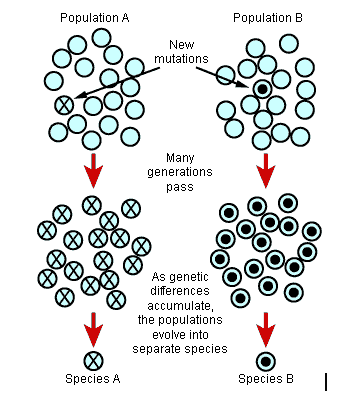
\includegraphics[width=0.7\textwidth]{figures/populations.png}
\end{center}
\caption{Simplified scheme of a speciation event in a population.} 
\end{figure}

In the early 1960s the first sequencing data became available from different groups of organisms. It was only a few small proteins, such as insulins\cite{Sanger1945}, hemoglobins\cite{INGRAM1956} and cytochrome c, but already then it became apparent that the evolution on the molecular level cannot only be explained by the adaptive processes\cite{King1969} and the mechanisms of introducing variety in the genome are not limited to mutation and recombination. A new field, molecular evolution emerged and new theories to explain the underlying processes of phenotypic diversity and genome size evolution were proposed.  
\section{Evolution of protein coding genes}
 Approaching evolutionary questions from the genotype perspective lead to the emergence of new theories of evolutionary mechanisms. Adaptive evolution driven by natural selection could not explain the overwhelming body of evidence for changes in the amino acids sequences that don't necessarily change the protein function, mutation rates on the sequence level and increase in genome size and complexity in high order organisms. 
 
 Kimura (1968)\cite{Kimura1968} and King and Jukes (1969)\cite{King1969} proposed that most mutant substitutions at the molecular level must be selectively neutral or nearly neutral, which created the alternative theory of neutral evolution. It has been controversial ever since, however, as more data is available from whole-genome sequencing of various species, it becomes clear that the general pattern of molecular evolution agrees with the neutral theory, even though some studies still suggest there are exceptions to the rule\cite{Haygood2007,Nielsen2007,Akey2009}  

Our knowledge about gene expression regulation in the genome has expanded significantly in the past 20 years. Since the landmark discovery of RNA interference, a process of small strands of RNA influencing gene expression, by Fire et.al \cite{Fire1998} many other regulatory mechanisms have been discovered.  The ENCODE consortium aiming to create a comprehensive encyclopedia of gene regulatory elements reports that even by the most conservative estimates at least 8.5\% of the bases in human genome are involved in direct gene regulation\cite{Bernstein2012}.  It is important, therefore, to study protein evolution in consideration of the regulatory elements in noncoding regions, non coding RNAs and other gene expression influences. However, because the function of most non coding regions is still poorly understood and the experimental data is sparse, in this research project we will focus mainly on the evolution of protein-coding genes. 

Let's introduce some of the main patterns of protein evolution with the key focus on introducing novelty to the genome.

\subsection{Protein sequence variations}
\subsubsection{Mutations}
Mutations are sequence changes at the DNA level and constitute the main origin for genetic diversity. For mutations to affect an organism's offspring, they must occur in cells that produce the next generation (as opposed to somatic mutations\cite{somatic}) and affect the hereditary material. In the smallest type of mutation event a single base pair in a DNA sequence is changed into another base pair. This type of mutations can lead to changes in the protein sequence if this segment or be synonymous, i.e., changed DNA segment will still code for the same amino acid. Synonymous mutations exist because many amino acids are encoded by multiple codons, as described in chapter 1.1.1. 

Mutations may also take the form of insertions or deletions, which are together known as indels. Number of nucleotide bases that is inserted or deleted from the DNA sequence can vary a lot. Indels of one or two bases in the coding sequences are the most common and can have a substantial impact on protein translation by causing a frameshift because of the triplet nature of codon expression.  

Based on the mutation's effect on fitness of the organism it can be beneficial, harmful or neutral. Beneficial or harmful mutations are what allows us to see natural selection in action. Mutation that increases the fitness of the organism and becomes heritable tends to increase in frequency in the population; harmful, or deleterious mutations, on the other hand, become extinct or stay at lower prevalence in the population. Neutral mutations don't have any effect on fitness and can become widely spread in a population and, according to the neutral theory, the majority of mutations that become fixed as differences between species are neutral. 

 Short indels that don't cause a frameshift in translation and become fixed in the population often occur in exposed loop regions\cite{Kim2010}. Longer indel events might involve an insertion or deletion of entire protein domain. The selective pressure acting on these events is less well understood, but fixed long indels are often associated with functional change\cite{Pascual-Garcia2010}.

\subsubsection{Gene duplication}
Gene duplication is agreeably the most important process for the generation of new genes during molecular evolution. During protein evolution analysis it is important to distinguish between the proteins that derived from a single ancestral gene in the last common ancestor of the given two species, i.e., as a result of a speciation event (orthologs), and proteins that evolved through duplication within the same (perhaps ancestral) genome, they are referred to as paralogs\cite{Jensen2001}.

There are at least two different ways in which it can occur: 
\begin{itemize} 
\item By duplication of a single gene or a group of genes 
\item By whole genome duplication 
\end{itemize}

The first of these mechanisms is the most common: multigene families are widely spread in all known species. By comparing the sequences of the members of these families it is possible to trace individual duplications that occurred in a common ancestral genome. Several mechanisms of these gene duplications are known in eukaryotes: unequal crossing-over, unequal sister chromatid exchange and replication slippage. The initial result of such an event is two identical genes. Selective constraints will ensure that one of these copies is still capable of maintaining the original function, the daughter copy in the meantime is subject to relaxed evolutionary pressure.

The majority of these excess gene copies acquire deleterious mutations that inactivate them so they become pseudogenes\cite{Zhang2001} Occasionally, though, the mutations that accumulate in this gene copy lead to a new function or a slightly altered sub-function of a parent gene.  Genes coding for different types of globin proteins that bind oxygen, evolved from a common ancestral gene which, after successive duplications and speciation events, led to the genes that encode the widespread globin superfamily\cite{Hardison1998}

Whole Genome Duplication (WGD) is the most rapid mechanism of increasing gene copy number and can occur due to an error during meiosis. The evidence from both experimental and computational studies\cite{Dehal2005} suggest that many gene innovations in yeast and animals result from WGDs during their evolutionary history. Increased complexity in the vertebrate developmental regulatory network is one of the important results of the two rounds of WGD at the base of vertebrate evolution\cite{Huminiecki2012}. 

\subsection{Protein structure and function constraints}
Evolution of animal phenotype is shaped by the selective pressures that might increase or reduce the benefits of acquired traits based on the cost inquired. Selective pressure may act on populations level (i.e., habitat conditions, population size), genome level (gene copy numbers, genome size) or molecular level. Strong evidence for selective pressure acting on protein evolution includes the fact that the three-dimensional structure tends to be more conserved than the corresponding amino acid sequence\cite{Illergard2009}. Strong structural constraints influencing protein evolution include maintenance of a hydrophobic core, secondary structure and charged hydrogen bonds.  
Additional constraints are added by protein-protein interactions\cite{Park2001} and differences in mutation rate for different proteins. For example, highly expressed proteins are constrained to have fewer mutations to avoid the cost of misfolding\cite{Subramanian2004}.  An understanding of the constraints on protein sequence variation is essential for understanding the mechanisms of protein evolution and need to be integrated in our further analysis. 

Most eukaryotic proteins consist of structural domains, each comprising a segment of the polypeptide chain corresponding to a certain fold in the three-dimensional structure. When studying duplication and rearrangement events in protein sequences it is important to keep this structural components in mind. Duplication of a whole structural domain might result in making a protein product more stable and therefore is under relaxed evolutionary pressure. The copy of the domain can change over time leading to a modified structure and protein activity. This evolutionary mechanism is particularly common in Metazoa\cite{Bjorklund2006} more often occur at the N and C-terminals\cite{Bjorklund2005} with the exception of protein repeats\cite{Bjorklund2006}, like in titin\cite{Higgins1994} and nebulin\cite{Bjorklund2010} proteins. 

 Domain shuffling is another result of a rearrangement event in the middle of a structural domain, it occurs when genes coding for different structural domains are joined  to form a new sequence coding for a hybrid protein, such an event can also lead to a novel combination of protein structure and function. Genes that are highly expressed in chordate structures, such as the endostyle, Reissner's fiber of the neural tube, and the notochord show evidence of domain shuffling during their evolution\cite{Kawashima2009}
 
\section{Protein disorder}
A notion that protein requires a rigid 3D structure to function has been prevalent ever since the 1931, when it was shown that protein denaturation leads to a complete loss of function\cite{Wu1995} This view has been somewhat challenged in the past 30 years. In 1970s the first unstructured, but functional region have been identified in fibrinogen; this region plays a key role in blood clotting\cite{Doolittle1973}. But up to the 1990s scientists were convinced that disordered regions they could observe by NMR spectroscopy are nothing more than artifacts. The structure of p21, discovered by Kriwacki to be fully disordered was something one could not deny any longer.  p21 was still able to perform its critical regulatory function even though although its amino acids never stayed in one conformation for more than a fraction of a second.
 
Several experimental approaches to identify intrinsically disordered regions in proteins have been developed or adapted from the existing ones since. In NMR chemical shifts analyses the pulse sequences have been tailored for resolving chemical shifts in the unfolded state, TROSY and CRINEPT-TROSY NMR spectroscopy now allow identifying the disorder-order transition during protein binding. Temperature and pressure dependent changes in the NMR results can indicate conformational fluctuation of disordered regions. NMR spin relaxation is also advancing to help characterize protein flexibility. H/D exchange in combination with mass spectrometry(HXMS) is used for high-throughput identification of disordered regions, since disordered regions have higher H/D exchange rates to be able to fold before binding with different partners\cite{Balasubramaniam2013}.  

Experimental identification of protein structure and disorder-to-order transition requires careful sample preparation and expensive equipment and are time consuming.  Here is where computational biology comes to the rescue. Based on the current knowledge of physical properties of protein disorder and amino acid sequences for experimentally identified unstructured regions several methods have been developed to predict disorder from protein sequence. On the basis of amino acid composition, hydropathy, capacity of polypeptides to form stabilizing contacts and other differences to known globular proteins these predictors label each amino acid in a protein sequence as ordered or disordered. While using these methods to study protein disorder and its evolution it is important to remember that they are limited to recognize patterns observed in experimentally verified disorder and each predictor is tailored to identify a certain type of characteristics\cite{Dunker2011}.

Roughly 30\% of human proteins are predicted to contain large intrinsically disordered regions. Many of these proteins perform critical functions in signaling, gene regulation and different protein interactions\cite{Iakoucheva2002}. Disordered regions are in our particular interest for this study also because they lack selective pressures against aggregation and misassembly described earlier, which can makes them subject to mutations altering protein function.  Intrinsic disorder was found to increase during evolution and correlates with organismal complexity\cite{Schlessinger2011,Xue2012}. Therefore protein disorder can be seen as yet another mechanism by which evolutionary novelty is created in protein evolution.  

\mychapter{2}{Materials and Methods}
\section{Databases}
\section{Computational methods}
 
\mychapter{3}{Projects}
\section{Expression pattern divergence between duplicated genes in mammals}

\section{Protein expansion is due to long indels in disordered regions}


\mychapter{4}{Future plans}
\section{Evolution of naturally disordered proteins}
 \section{Evolution of long insertions and deletions in different domains of life}

\bibliographystyle{abbrv}
\bibliography{references}

\end{document}

